\chapter{RFID Microcontroller}
\section{Introduction}
The \gls{rfid} microcontroller is a versatile and compact system designed to interface with \gls{rfid} readers and process tag information efficiently. It acts as a bridge between \gls{rfid} 
hardware and software applications, enabling seamless communication and data exchange. Built around the NodeMCU, which is powered by the ESP8266 chip, the microcontroller 
offers robust processing capabilities and integrated \gls{wifi} connectivity. This makes it ideal for \gls{iot} applications where \gls{rfid} data needs to be transmitted over a network for further 
processing, monitoring, or storage. The system is designed to be reliable, scalable, and easy to integrate into various use cases, including access control, inventory management, asset tracking, 
and smart automation systems.
\section{Hardware}
\subsection{Schematic}
The schematic diagram in Figure \ref{fig:rfid-schematic} illustrates the design of the \gls{rfid} microcontroller circuit. It shows the connections between componentse and the terminal blocks for one or two \gls{rfid} readers. 
Each component is carefully integrated to ensure reliable recieving the tag information from the \gls{rfid} readers.

\begin{figure}[H]
  \centering
    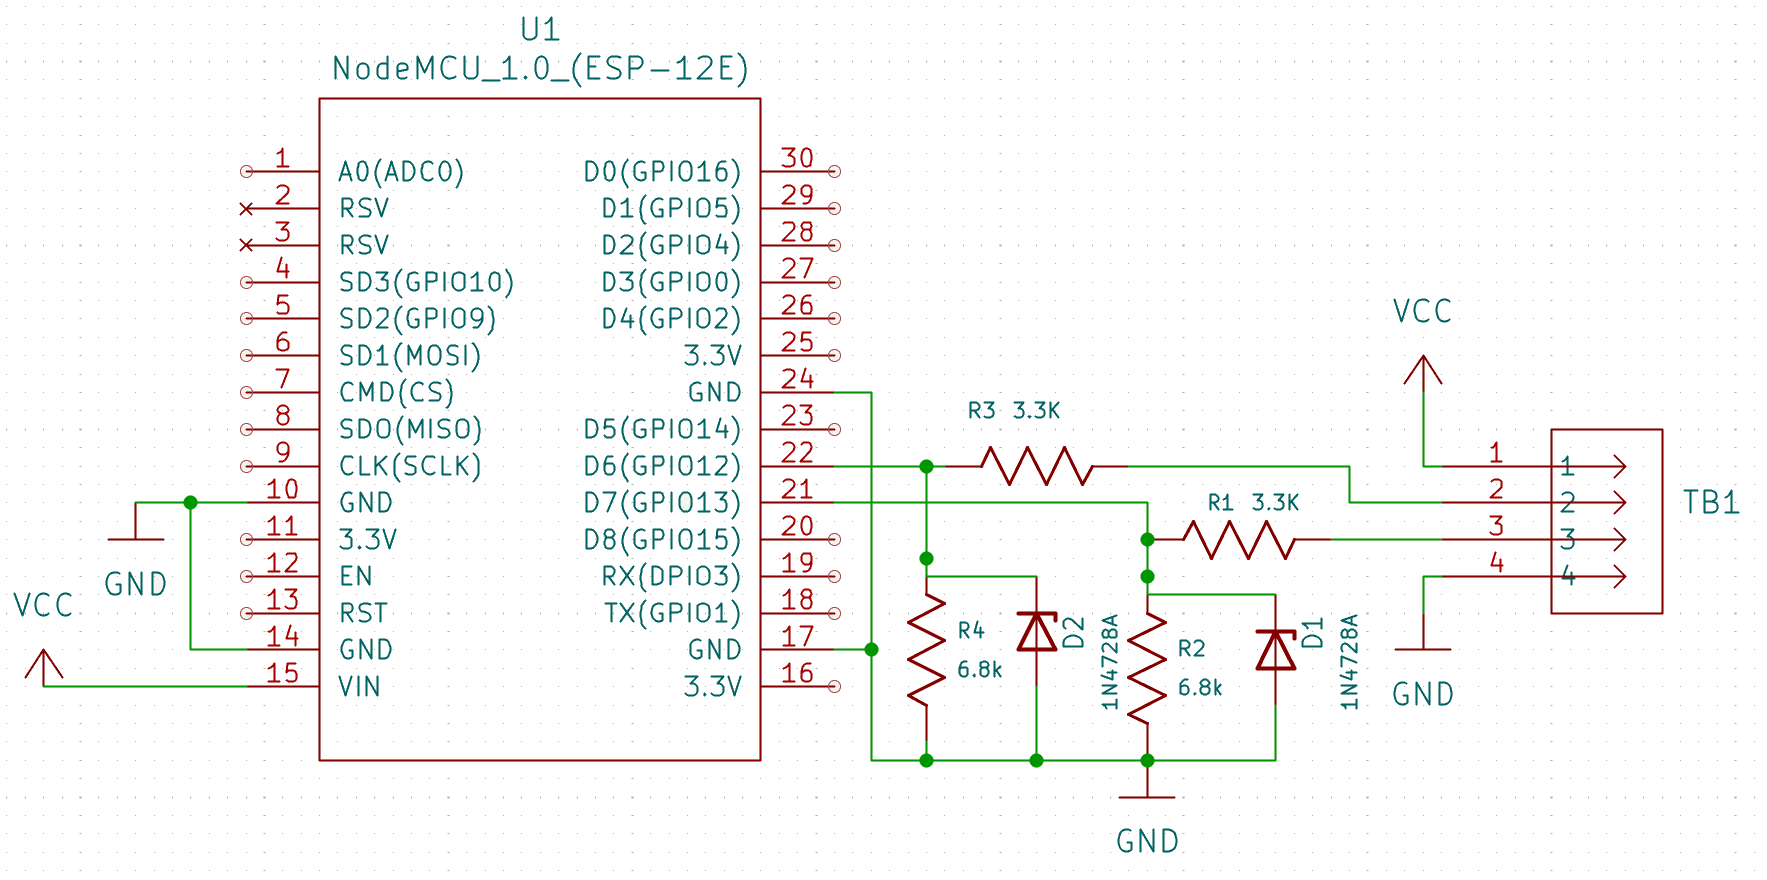
\includegraphics[scale=0.2]{../Images/rfid_schematic.png}
  \caption{RFID Microcontroller Schematic}
  \label{fig:rfid-schematic}
\end{figure}

The hardware used in the \gls{rfid} microcontroller circuit consists of several components that work together to enable the \gls{rfid} readers. The main components are:
\begin{itemize}
\item NodeMCU (U1) is the central microcontroller, an ESP8266, which will manage communication with the \gls{rfid} readers.
\item Resistors (R1, R2, R3, R4) are resistors crucial for voltage level shifting.
\item Zener Diodes (D1, D2) are diodes, along with the resistors, form a level shifting circuit.
\item TB1 Connector is the 4-pin connector where the \gls{rfid} readers are attached.
\end{itemize}
The NodeMCU (U1) is programmed to handle the communication with the \gls{rfid} readers through the \gls{i2c} protocol. The resistors (R1, R2, R3, and R4) are used in a level shifting circuit to ensure that the voltage levels between the 
NodeMCU and the \gls{rfid} readers are compatible. The diodes (D1 and D2) are used to protect against voltage spikes and ensure proper operation of the level shifting circuit. The TB1 connector is where the \gls{rfid} readers are connected to the microcontroller.

\subsection{PCB Design}
The \gls{pcb} design for the \gls{rfid} microcontroller is shown in Figure \ref{fig:rfid_pcb}. The PCB layout is designed to accommodate all the components mentioned in the schematic, ensuring proper 
connections and efficient routing of signals.

\begin{figure}[H]
  \centering
    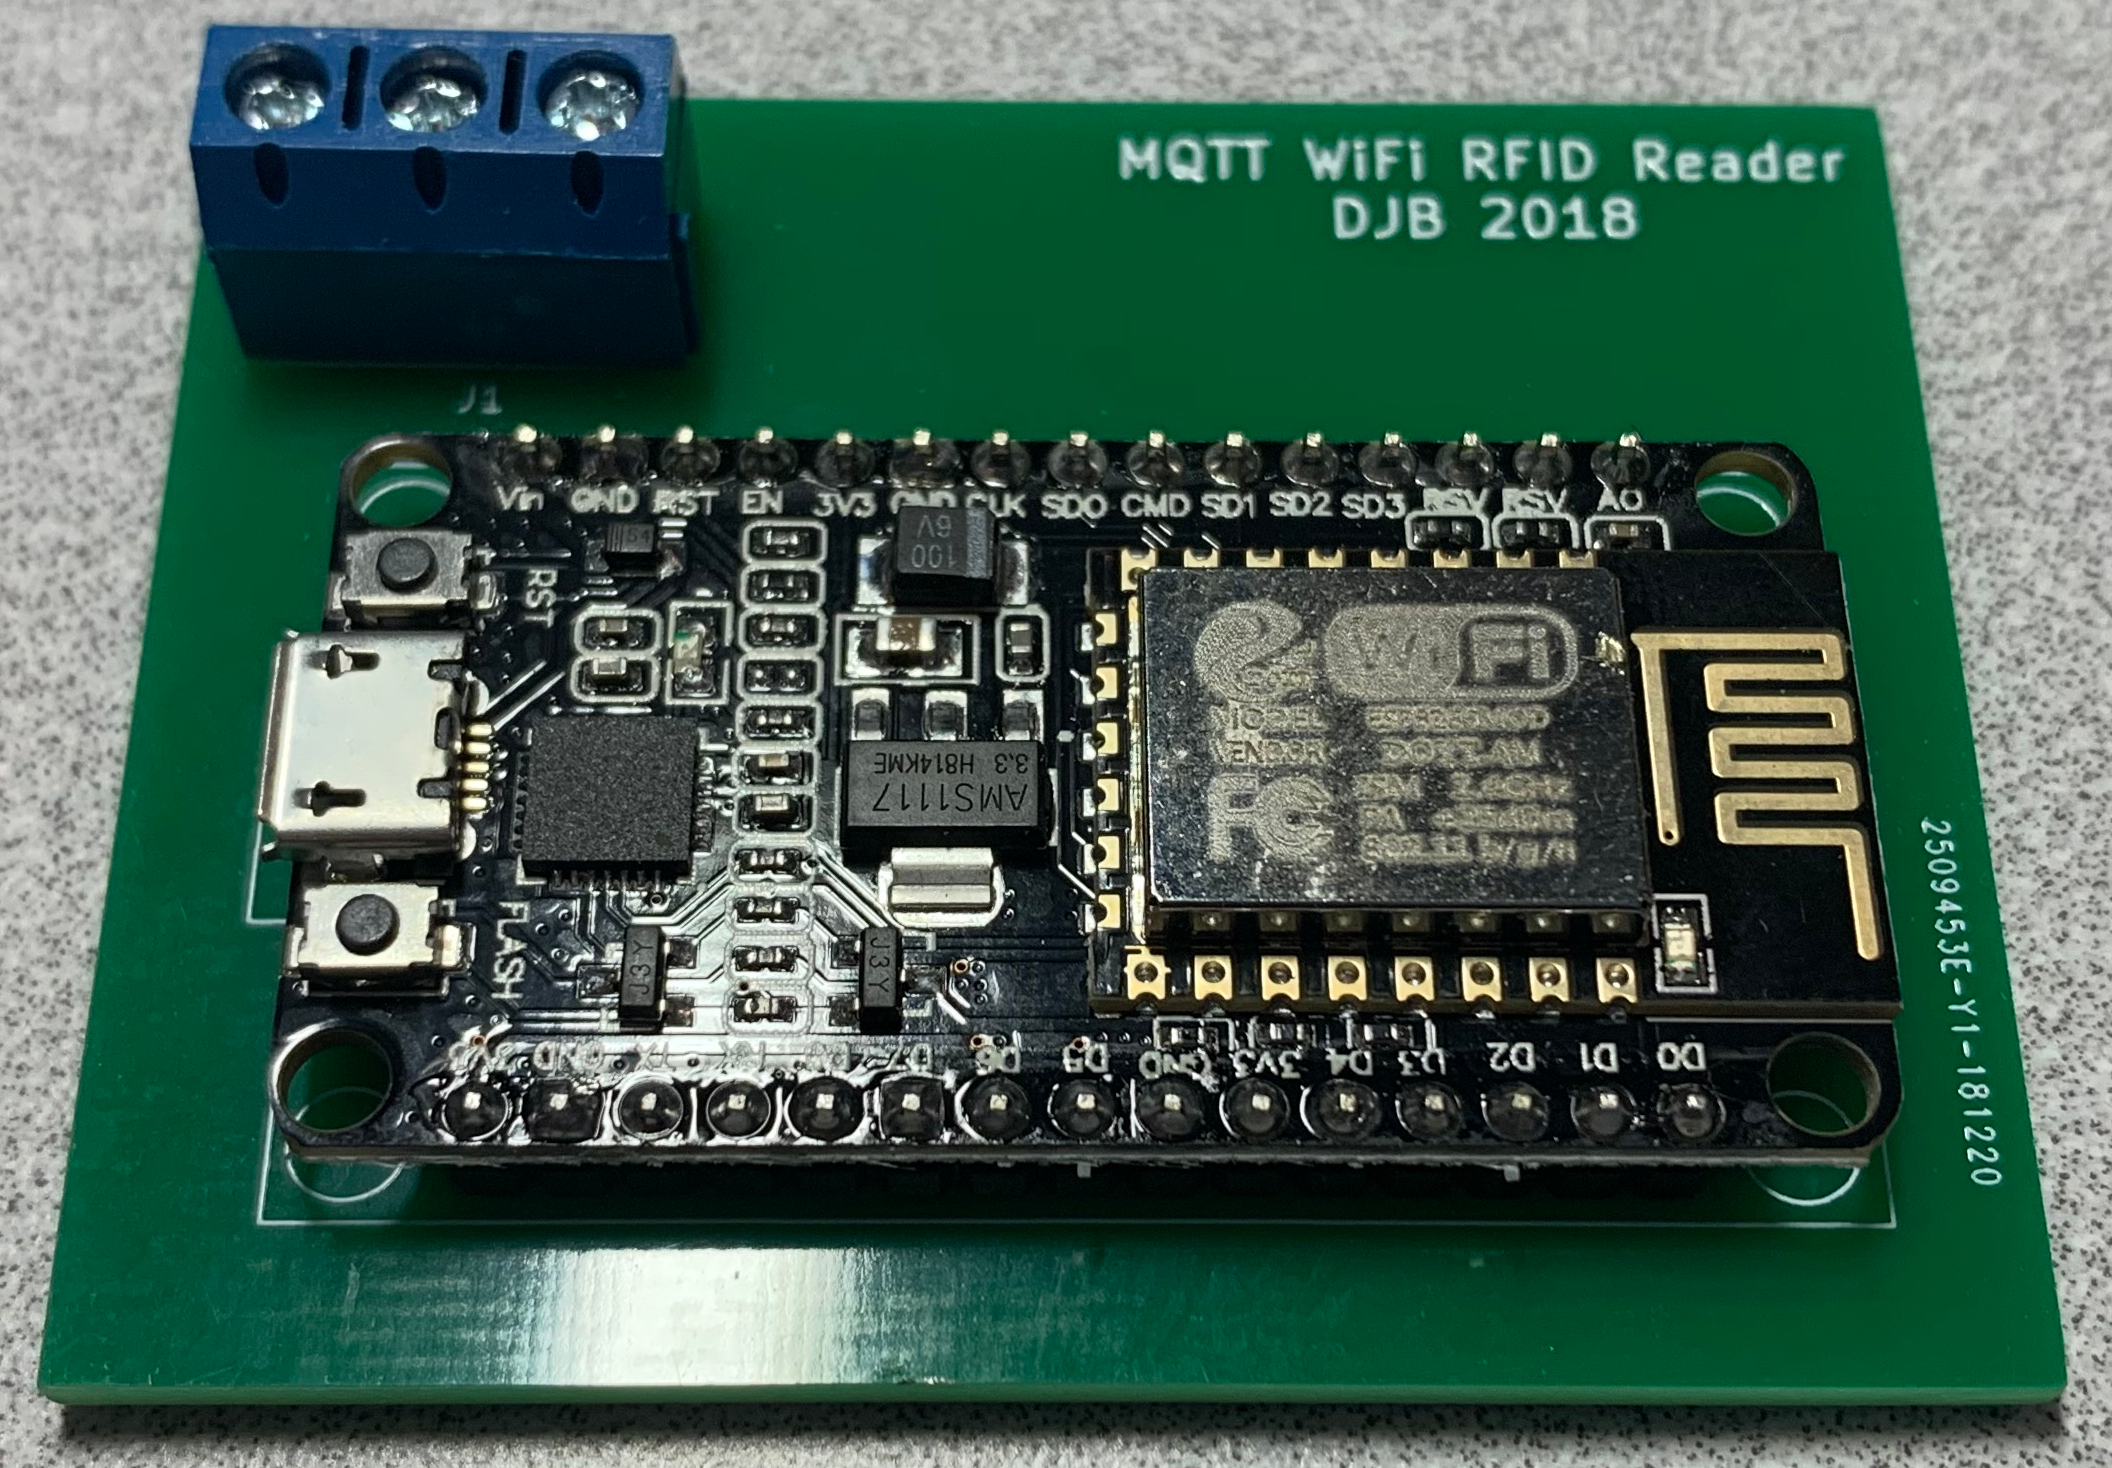
\includegraphics[scale=0.15]{../Images/rfid_pcb.png}
  \caption{RFID Microcontroller PCB}
  \label{fig:rfid_pcb}
\end{figure}
\subsection{Connectivity}
The wiring diagram in Figure \ref{fig:rfid-board} illustrates the connections between the \gls{rfid} readers and the microcontroller. The \gls{rfid} readers are connected to the TB1 terminal block, which uses a RS232 connection to the NodeMCU.
The connections are made using standard wiring techniques, ensuring reliable and secure connections. The use of terminal blocks allows for easy connection and disconnection of the Tortoise machines, making maintenance and troubleshooting easier.
\begin{figure}[H]
  \centering
    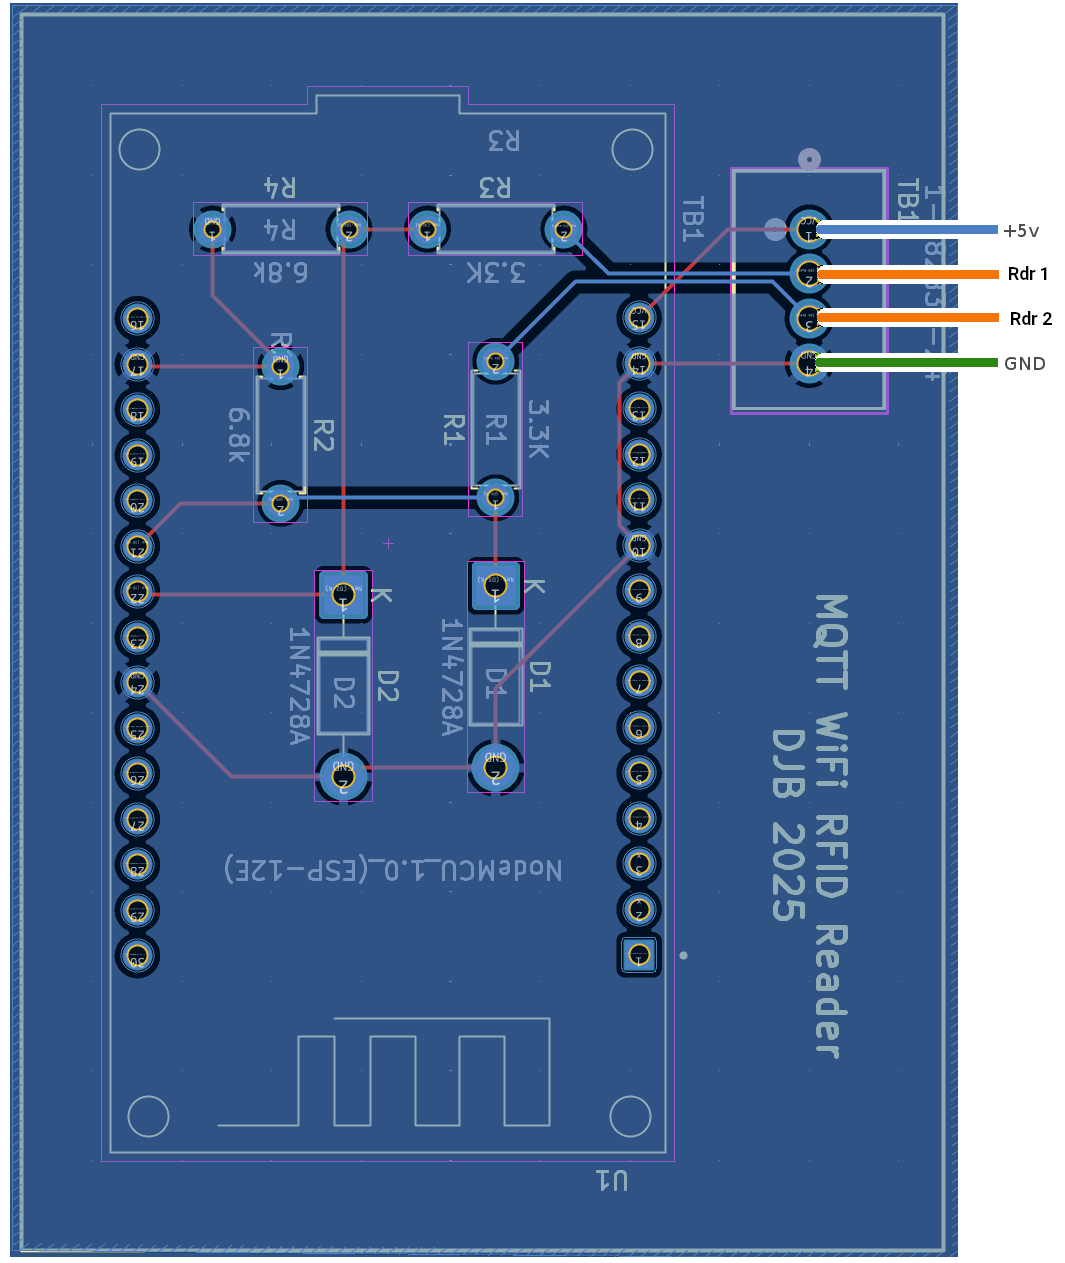
\includegraphics[scale=0.2]{../Images/rfid-board.png}\hfill
    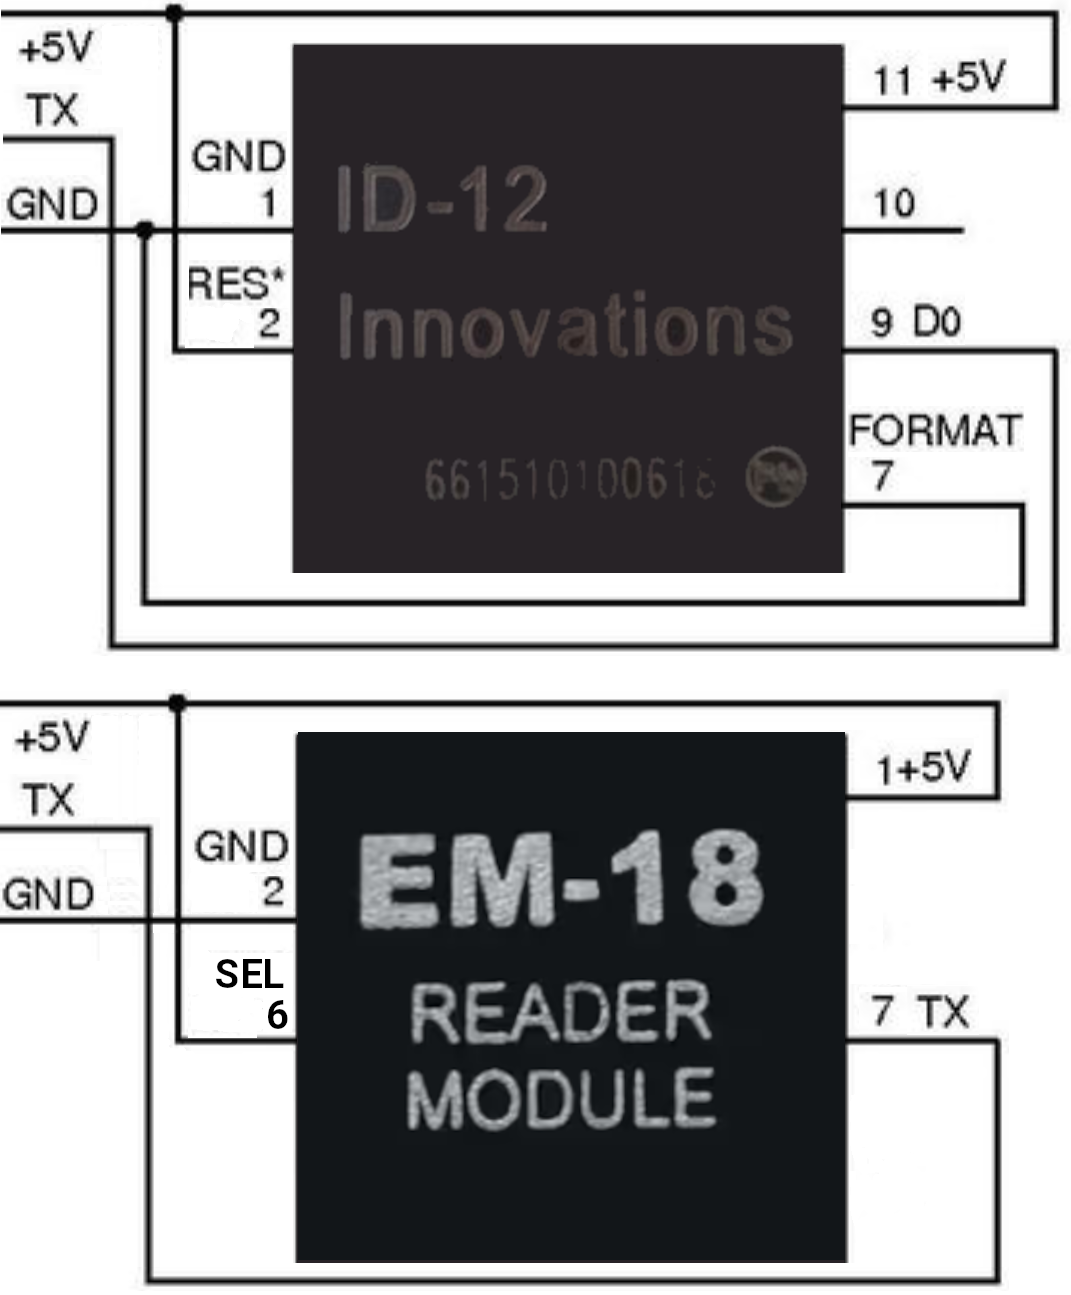
\includegraphics[scale=0.2]{../Images/rfid-readers.png}
  \caption{RFID Microcontroller - RFID Reader Connections}
  \label{fig:rfid-board}
\end{figure}

\section{Software}
The software for the \gls{rfid} microcontroller is developed using the \gls{vscode}, which provides a user-friendly environment for programming microcontrollers. The code is written in C/C++ and utilizes various libraries to facilitate communication with the components.
The software implementation includes the following key functionalities:
\begin{itemize}
  \item Initialization of the NodeMCU and configuration of the GPIO pins.
  \item Initialization of the \gls{wifi} connectivity and connect to the \gls{mqtt} broker. This allows the microcontroller to send and receive messages over the network.
  At the finish of the initialization process, the microcontroller, it will publish a message to the topic ``micros'' indicating its readiness and status to the \gls{mqtt} broker. The message is in \gls{json} format as follows:\\
  \{``et'':``1590462747'',``mcntrlr'':``RfidRdr01'',``msgType'':``initial'',``ip'':``192.168.0.19''\}
\item Setup of the serial communication protocol to interface with the \gls{rfid} reader module. This allows for reading \gls{rfid} tags.
\item Handling \gls{rfid} tag detection and processing the data received from the \gls{rfid} reader. reads values from a single \gls{rfid} reader, formats the results as a \gls{json} string, gets Epoch time from an NTP server and then publishes the \gls{json} String to the topic ``sensors/rfid'' on the \gls{mqtt} broker. The message is in \gls{json} format as follows:\\
\{``et'':``1590463450'',``mcntrlr'':``RfidRdr01'',``reader'':``1'',``rfid'':``1C0044CF23''\}
\item Sending periodic heartbeat messages to the \gls{mqtt} broker to indicate that the microcontroller is operational. This can be used for monitoring and debugging purposes. The message are in \gls{json} format as follows:\\
\{``et'':``1590462747'',``mcntrlr'':``RfidRdr01'',``msgType'':``heartbeat''\}
\end{itemize}
The software is designed to be modular and easily maintainable, allowing for future enhancements and bug fixes. The use of libraries such as ``PubSubClient.h'' for \gls{mqtt} messaging simplifies the implementation and ensures compatibility with the hardware components.
